\section{Results}\label{sec:results}

\subsection{The mechanism at full range}\label{sec:sweep}

Figure~\ref{fig:sweep-rev} runs the composition mechanism from 0\% to 100\%.
Net government revenue falls almost monotonically as labor income becomes
capital income, bottoming at \genSweepTroughRev B at a
\genSweepTroughShift\% shift. The decomposition is not what a
``capital-is-taxed-lightly'' intuition alone would predict: the federal
income tax \emph{gains} at every step (\genSweepTenIIT B at the first),
because concentrating income into the small capital-holding population
pushes it into upper brackets by more than the preferential rates give back.
Revenue falls anyway because payroll collections fall roughly linearly with
the wage base (\genSweepTenPayroll B at the first step) and benefit outlays
and refundable
credits rise as wage-dependent households qualify for means-tested support;
state codes track the federal income-tax pattern.
The distributional counterpart (Figure~\ref{fig:sweep-dist}) is severe by
construction --- only \genSweepHHCapSharePct\% of households hold any
positive capital income, so the net-income Gini rises from
\genSweepBaseGini{} to \genSweepFullGini{} and SPM poverty from
\genSweepBasePovPct\% to \genSweepFullPovPct\% at the full shift, with the
top decile's mean net income rising \genSweepTopDecilePct\% while decile
\genSweepWorstDecile{} falls \genSweepWorstDecilePct\%. The exception is
instructive and is the transfer system's signature: the bottom decile ends
essentially where it started (\genSweepBottomDecilePct\%), because its income
is largely transfers, which do not follow wages out of the labor market. The
forecast-equivalent range --- the shaded band at
\genForecastShiftSlowPct{}--\genForecastShiftRapidPct\% --- says how much of
this axis the 2030 forecasts actually reach: the first decade. The sweep's
value is the mechanism it exposes, not the tail. These sweep runs predate the
correction noted before the introduction: their benefit outlays and net
income still include Head Start and Early Head Start.

\begin{figure}[t]
\centering
\includegraphics[width=0.92\textwidth]{figures/sweep_revenue.pdf}
\caption{Revenue under a 0--100\% labor-to-capital shift,
\genSweepYear{}. Lines are changes against baseline; benefit outlays are
sign-flipped so a rising line is a fiscal cost. The shaded band marks the
forecast-equivalent positions of the 2030 scenarios.}
\label{fig:sweep-rev}
\end{figure}

\begin{figure}[t]
\centering
\includegraphics[width=0.92\textwidth]{figures/sweep_distribution.pdf}
\caption{Inequality and poverty under the same sweep.}
\label{fig:sweep-dist}
\end{figure}

\subsection{Calibrated scenarios}\label{sec:scenarios}

Table~\ref{tab:grid} reports all twelve scenario cells at 2030 against the
same-year current-law baseline; Figure~\ref{fig:scenarios} plots the Rapid
pattern. Two published Budget Lab mechanisms reproduce on independent
machinery. Within each scenario, moving from compressive to expansive raises
income-tax revenue through progressivity and lowers payroll revenue as
earnings cross the Social Security taxable maximum. And the tilt is
expensive: Table~\ref{tab:tilt} shows each scenario keeping a fraction of its
shares-fixed revenue --- \genKeptHouseholdRapidPct\% in Rapid
(\genRapidPropRev B against \genRapidFixedRev B) on this all-government
household basis, against \genKeptMatchedRapidPct\% on the narrower federal
basis Section~\ref{sec:reconciliation} matches to the Budget Lab. The
difference between those two keep-rates is mainly the Budget Lab's corporate
wedge, which the federal basis includes: it grows with the capital shock, so
it cushions the as-forecast cell. The state and transfer channels add to the
tilt's dollar cost but leave the keep-rate essentially unchanged.

\begin{table}[t]
\centering
\small
\tabScenarioGrid
\caption{Scenario grid, 2030, \$B change against the current-law baseline
(SPM poverty \genBaselinePovertyPct\%, net Gini \genBaselineGini{}).
``Revenue'' is net government revenue (federal and state taxes minus
refundable credits and benefits); ``Income tax'' is federal income tax
gross of refundable credits; ``State'' is state tax before refundable state
credits.}
\label{tab:grid}
\end{table}

\begin{table}[t]
\centering
\tabTilt
\caption{What the tilt toward capital costs: net revenue with factor shares
fixed versus as forecast (proportional wage spread), \$B, 2030.}
\label{tab:tilt}
\end{table}

\begin{figure}[t]
\centering
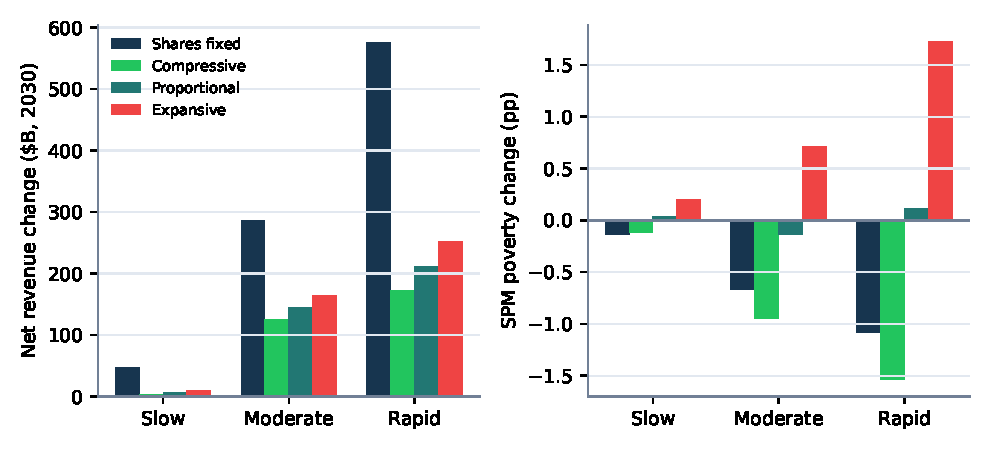
\includegraphics[width=0.95\textwidth]{figures/scenarios.pdf}
\caption{Net revenue (left) and SPM poverty change (right) by scenario and
wage-inequality variant, 2030.}
\label{fig:scenarios}
\end{figure}

The payroll-cap mechanism runs in both directions, which is worth stating
because it is easy to get backwards: under Rapid~/~compressive, aggregate
labor income \emph{falls} \genRapidCompLaborPct\% and payroll receipts still
\emph{rise} \genRapidCompPayroll B, because compression moves earnings from
above the taxable maximum to below it; under expansive the same cap turns
wage growth into a payroll loss of \genRapidExpPayroll B. The wage-spread
parameter also has a direct household reading: each variant has a crossover
wage below which workers lose (expansive,
\$\genRapidExpCrossover{}) or gain (compressive,
\$\genRapidCompCrossover{}), so under Rapid~/~expansive the great majority of
workers sit on the losing side of a scenario that adds \genRapidExpRev B to
net revenue.

\subsection{The transfer system}\label{sec:transfers}

The Revenue column of Table~\ref{tab:grid} nets transfers out; pulling them
apart shows the safety net responding exactly as designed
(Figure~\ref{fig:transfers}). Across the Rapid wage-spread variants ---
identical aggregate labor income, only its distribution varies --- gross tax
collections swing \$\genGrossTaxSwing B, and automatic transfer responses
absorb \$\genTransferSwing B of that swing, \genTransferAbsorbPct\%.
Non-credit transfers alone swing \$\genBenefitSwing B: \genRapidCompBenefits
B under compressive, as rising low-end wages float households off
means-tested programs, to \genRapidExpBenefits B under expansive as falling
ones push them on. SNAP carries \$\genSnapSwing B of the swing
(\genRapidCompSnap B to \genRapidExpSnap B) and SSI \$\genSsiSwing B;
Moderate shows the same shape (\genModCompBenefits B to \genModExpBenefits
B). Refundable credits contribute the remaining \$\genCreditSwing B --- a
response the Budget Lab's accounting does capture through its tax-credit
outlays line. The \$\genBenefitSwing B of program spending is the piece
outside their model's coverage, and it is the outlay side of the
\genRapidPovSpanPp pp poverty span: the same variant uncertainty their
report scores as a revenue question arrives at households as a benefits
question.

\begin{figure}[t]
\centering
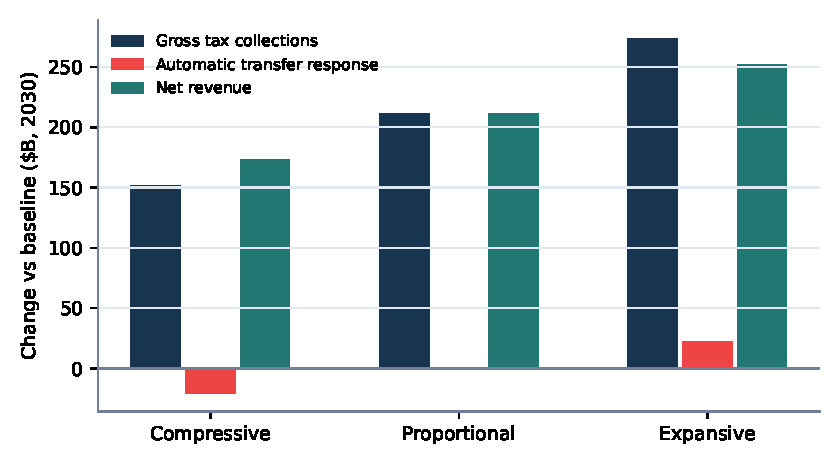
\includegraphics[width=0.8\textwidth]{figures/transfers.pdf}
\caption{Gross tax collections, automatic transfer response, and net revenue
across the Rapid wage-inequality variants, 2030. Transfers (refundable
credits plus benefits) rise exactly when workers lose, absorbing
\genTransferAbsorbPct\% of the gross-tax swing across the variants.}
\label{fig:transfers}
\end{figure}

\subsection{States}\label{sec:states}

State codes are the other channel a federal model does not carry. Under
Rapid~/~proportional they collect \genRapidPropState B, and the state take
doubles across the wage-spread variants (\genRapidCompState B to
\genRapidExpState B) as progressive state schedules concentrate collections
at the top the way federal brackets do. On the Rapid~/~expansive cell used
for the reconciliation below, state tax net of refundable state credits adds
\genRapidExpStateNet B --- roughly a sixth on top of the bridged federal
take.

The geography is concentrated (Figure~\ref{fig:states}): the top five states
collect \genStateTopFiveSharePct\% of the national state take
(\genStateFirst, \genStateSecond, \genStateThird, \genStateFourth,
\genStateFifth, in \$B). \genNZeroStates{} states collect exactly nothing
from the capital shock --- \genZeroStatesList{} --- and Washington is the
instructive exception: it has no income tax either, but its capital-gains excise tax
collects \genWAState B, more than the seven zero-collecting states combined.
A state that taxes capital gains participates in an AI capital boom; a state
that taxes only wages does not participate in an economy where wages are the
shrinking share. State-funded benefit responses are negligible in these runs
(the model's state-benefit registry at version \genModelVersion{} covers
state SSI supplements and child-care subsidies), so the automatic-stabilizer
response above is almost entirely federal. Sub-national cells this small
carry material data-calibration sensitivity --- Section~\ref{sec:stability}
shows a single data-build revision moving New York's take from
\$\genStabNYOld B to \$\genStabNYNew B --- so the state figures locate the
pattern rather than measure any one state precisely.

\begin{figure}[t]
\centering
\includegraphics[width=0.8\textwidth]{figures/states.pdf}
\caption{Top ten states by net state revenue change, Rapid~/~proportional,
2030.}
\label{fig:states}
\end{figure}
